\documentclass[final]{these-ISSS}

\usepackage{mesmacros}



\titre{Pourquoi les macarons de Ladurée sont-ils si bons ?}
%\soustitre{C'est si bon}
\title{Why Ladurée macarons are so good?}
\firstname{Pierre}
\lastname{Hermé}
%\laboratoire{} %Déclaration du nom du labo si ce n'est pas l'I3S
%\cotutelle{Université de la Pâtisserie} % Ajouter une cotutelle si elle existe
%\cotutellelogo{Pastry_Bag.png}
\date{} % Mettre la date de soutenance
\discipline{Pâtisserie} % Informatique par défaut
%\cofinanceurslogo{Pastry_Bag.png, Pastry_Bag.png, Pastry_Bag.png}
%\hdr




\begin{document}
  \pagenumbering{roman}  
  
  
\begin{jury}[Paul \Nom{Bocuse}, Grand chef cuisinier/L'Auberge du Pont de Collonges]%% Mettre ici le nom du président
%% Autant de lignes \rapporteur que nécessaire
%% Autant de lignes \examinateur que nécessaire
  \rapporteur{Patrick \Nom{Lenôtre}}{Chef de cuisine}{Pavillon des Princes, Paris}
  \rapporteur{Christophe \Nom{Michalak}}{Chef pâtissier}{l'Hôtel Plaza-Athénée, Paris}
  \examinateur{Cédric \Nom{Grolet}}{Chef pâtissier}{Le Meurice}
  \invite{Michel \Nom{Guérard}}{Cuisinier}{Les Prés d'Eugénie}
  \directeur{Jean-Paul \Nom{Hévin}}
  \codirecteur{Antoine \Nom{Santos}}
  \coencadrant{Laurent \Nom{Duchêne}}
\end{jury}

  
  \maketitle

  \begin{dedicace}
    À toi lecteur <3 :*
  \end{dedicace}

  \cleardoublepage
  
  
%%------------------------------------------------ Le résumé et les mots-clés -
\begin{ResumeMotsCles}
%% Résumé en français : pas plus de 2000 caractères
\begin{resume}
Les macarons c'est bon par nature, c'est le propre même du macaron que d'être bon. Au vue de l'affluence constante aux divers magasins Ladurée on peut supposer que les macarons qu'on y trouve sont meilleurs qu'ailleurs. Cette thèse vise à donner des idées et pistes sur le pourquoi du comment que les macarons de Ladurée sont si bons.
\end{resume}

%% Résumé en anglais : pas plus de 2000 caractères
\begin{abstract}
Macarons are so good.
\end{abstract}

%% Mots-clés en français
\motscles{Pâtisserie, Macaron, Ladurée.}
%% Mots-clés en anglais
\keywords{Pastry, Macaron, Ladurée.}
\end{ResumeMotsCles}

  
  
\begin{remerciements}
Merci !
\end{remerciements}


  \tableofcontents

  \mainmatter

  % !TEX root = ../sommaire.tex

\chapter{Introduction}

\section{Contexte}

\section{Présentation de la problématique}

\section{Organisation de ce manuscrit}

\section{Nos contributions}



  % !TEX root = sommaire.tex
\Chapter{Notations}

\section*{P\^atisserie}

\begin{tabular}{p{2cm} p{11.5cm}}
  \hline
  $\mathcal{D}$ & l'ensemble des donuts\\
  $\mathcal{M}$ & l'ensemble des macarons\\
  $d_i$ & le donut $i$\\
  $m_i$ & le macaron $i$\\
  \hline
\end{tabular}

\section*{Viennoiserie}

\begin{tabular}{p{2cm} p{11.5cm}}
  \hline
  $\mathcal{V}$ & l'ensemble des viennoiseries\\
  $\mathcal{C}$ & l'ensemble des croissants\\
  $v_i$ & la viennoiserie $i$\\
  $c_i$ & le croissant $i$\\
  \hline
\end{tabular}


  \Part{État de l'art}
  % !TEX root = ../sommaire.tex

\chapter{La Pâtisserie}

% !TEX root = ../sommaire.tex

\chapres{\lipsum[1]}{\lipsum[2]}

% !TEX root = ../sommaire.tex

\section{La pâtisserie de la préhistoire à aujourd'hui}

Comme chacun sait la pâtisserie a toujours existé, même les hommes et femmes préhistoriques aimaient finir leurs repas sur une note sucrée.

\subsection{Les premiers gâteaux}


\subsubsection{La première tarte}

Rappelons d'abord la définition de la tarte telle que donnée dans \cite{S2012}.

\begin{definition}[Tarte]
  Une tarte, c'est comme un donuts mais sans trous et avec des fois des fruits dessus.
\end{definition}

\begin{example}[Tarte]
  La tarte aux citrons et une tarte.
\end{example}

\begin{remark}
  Notons que la tarte au chocolat est aussi une tarte par contre le mille-feuilles n'est pas une tarte.
\end{remark}

Après de très nombreux travaux on peut aujourd'hui affirmer que la première tarte était une tarte aux citrons, et vous devez nous croire parce qu'on porte des lunettes de soleil \cite{C2012}.

\subsubsection{Le premier éclair}

\subsubsection{Le premier flan}

\subsubsection{La première religieuse}


\subsection{Évolution de la pâtisserie au cours du temps}

\subsection{L'arrivée du Macaron}

\subsection{Conclusion}

\section{La pâtisserie dans le monde}


\subsection{Pâtisserie suédoise}
Les suédois font \emph{fika} pour le plaisir de tous.

\subsection{Pâtisserie orientale}
Toutes ces pâtisseries très sucrées à la pistache qui sont très très bonnes.

\subsection{Pâtisserie anglaise}
Non c'est une blague :) \cite{F2011}

\subsection{Conclusion}

\section{Synthèse}


\subsection{La place du macaron dans le monde}

\subsection{Analyse}

  % !TEX root = ../sommaire.tex

\chapter{Les macarons c'est bon}

% !TEX root = ../sommaire.tex

\chapres{\lipsum[1]}{\lipsum[2]}

%%%%%%%%%%%%%%%%%%%%%%%%%%%%%
\section{Introduction}
%%%%%%%%%%%%%%%%%%%%%%%%%%%%%

%%%%%%%%%%%%%%%%%%%%%%%%%%%%%
\section{Les macarons}
%%%%%%%%%%%%%%%%%%%%%%%%%%%%%
\begin{definition}[Macaron]
  Les macarons c'est de petits gâteaux à base de meringue qui sont très bons.
  \label{def:macaron}
\end{definition}

\begin{proposition}
  Les macarons c'est bon.
\end{proposition}

\begin{proof}
  Montrons que macarons $\Leftrightarrow$ bon
  
  \begin{myproof}[macaron $\Rightarrow$ bon]
    Preuve direct par définition \ref{def:macaron} (\nameref{def:macaron}).
  \end{myproof}
  \begin{myproof}[macaron $\Leftarrow$ bon]
    Preuve un peu plus tricky mais bon croyez nous quand on vous dit que c'est bon.
  \end{myproof}
  Donc les macarons sont bons.
\end{proof}

%%%%%%%%%%%%%%%%%%%%%%%%%%%%%
\section{Conclusion}
%%%%%%%%%%%%%%%%%%%%%%%%%%%%%


  \Part{Contributions}
  % !TEX root = ../sommaire.tex

\chapter{Chapitre 4}

\chaptoc

%%%%%%%%%%%%%%%%%%%%%%%%%%%%%
\section{Section 1}
%%%%%%%%%%%%%%%%%%%%%%%%%%%%%

\begin{figure}
  \centering
  \subfigure[subfigure 1]{\label{fig:subfig1}
    \begin{tikzpicture}
      \fill [black] (-1.25, -1.25) rectangle (1.25, 1.25); 
      \begin{scope}
        \clip (-1, -1) rectangle (0, 0);
        \fill[purple] (0,0) circle (1);
      \end{scope}
      \begin{scope}
        \clip (-1, 0) rectangle (0, 1);
        \fill[bleu] (0,0) circle (1);
      \end{scope}
      \begin{scope}
        \clip (0, 0) rectangle (1, 1);
        \fill[pink] (0,0) circle (1);
      \end{scope}
      \begin{scope}
        \clip (0, -1) rectangle (1, 0);
        \fill[vert] (0,0) circle (1);
      \end{scope}
    \end{tikzpicture}}
  \subfigure[subfigure 2]{\label{fig:subfig2}
    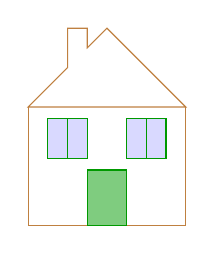
\begin{tikzpicture}
      \draw[brown] (0, 0) -- (0.5, 0.5) -- (0.5, 1) -- (0.75, 1) -- (0.75, 0.75) -- (1, 1) -- (2, 0) -- cycle;
      \draw[brown] (0, 0) -- (0, -1.5) -- (2, -1.5) --  (2, 0);
      \draw[color = green!60!black, fill = blue, fill opacity = 0.15] (0.25, -0.65) rectangle (0.75, -0.15);
      \draw[color = green!60!black, fill = blue, fill opacity = 0.15] (1.25, -0.65) rectangle (1.75, -0.15);
      \draw[color = green!60!black] (0.5, -0.65) -- (0.5, -0.15);
      \draw[color = green!60!black] (1.5, -0.65) -- (1.5, -0.15);
      \filldraw[color = green!60!black, fill opacity = 0.5] (0.75, -1.5) rectangle (1.25, -0.8);
    \end{tikzpicture}}
  \caption[Dessins]{Subfigure 1 \ref{fig:subfig1} et subfigure 2 \ref{fig:subfig2}.}
  \label{fig:figure1}
\end{figure}

La figure \ref{fig:figure1} est vraiment magnifique. Elle est composée des sous-figures \ref{fig:subfig1} et \ref{fig:subfig2}.

%%%%%%%%%%%%%%%%%%%%%%%%%%%%%
\section{Section 2}
%%%%%%%%%%%%%%%%%%%%%%%%%%%%%

\begin{algorithm}
  \begin{algorithmic}
    \STATE tableau d'entiers tab \COMMENT{tableau d'entiers}
    \STATE int $i$ \COMMENT{indice de parcours}
    \STATE int $m$ \COMMENT{valeur maximale du tableau}
    \STATE
    \STATE $m \leftarrow$ tab[1]
    \FOR{$i$ \FROM 2 \TO length(tab)}
      \IF{$m <$ tab[$i$]}
        \STATE $m \leftarrow$ tab[$i$]
      \ENDIF
    \ENDFOR
  \end{algorithmic}
  \caption[Algorithme 1]{Met dans $m$ la valeur maximale du tableau tab.\label{ag:algo1}}
\end{algorithm}

L'algorithme \ref{ag:algo1} utilise le package algorithmic.

%%%%%%%%%%%%%%%%%%%%%%%%%%%%%
\section{Section 3}
%%%%%%%%%%%%%%%%%%%%%%%%%%%%%

La section 3.

%%%%%%%%%%%%%%%%%%%%%%%%%%%%%
\section{Conclusion}
%%%%%%%%%%%%%%%%%%%%%%%%%%%%%
  % !TEX root = ../sommaire.tex

\chapter{Chapitre 5}

% !TEX root = ../sommaire.tex

\chapres{\lipsum[1]}{\lipsum[2]}

\tikzstyle{nodedefault} = [draw, circle]
\tikzstyle{edgedefault} = [draw]

\tikzstyle{n1} = [nodedefault]
\tikzstyle{n2} = [nodedefault]
\tikzstyle{n3} = [nodedefault]
\tikzstyle{n4} = [nodedefault]
\tikzstyle{n5} = [nodedefault]
\tikzstyle{n6} = [nodedefault]
\tikzstyle{n7} = [nodedefault]
\tikzstyle{n8} = [nodedefault]
\tikzstyle{n9} = [nodedefault]

\tikzstyle{a12} = [edgedefault]
\tikzstyle{a13} = [edgedefault]
\tikzstyle{a25} = [edgedefault]
\tikzstyle{a34} = [edgedefault]
\tikzstyle{a46} = [edgedefault]
\tikzstyle{a56} = [edgedefault]
\tikzstyle{a67} = [edgedefault]
\tikzstyle{a68} = [edgedefault]
\tikzstyle{a79} = [edgedefault]
\tikzstyle{a89} = [edgedefault]

% style pour les noeuds roses
\tikzstyle{nrose} = [pink]

% style pour les noeuds bleus
\tikzstyle{nbleu} = [white, fill = bleu]

%%%%%%%%%%%%%%%%%%%%%%%%%%%%%
\section{Section 1}
%%%%%%%%%%%%%%%%%%%%%%%%%%%%%

\begin{figure}
  \centering
    
  \begin{tikzpicture}[every node/.style = {nodedefault}, every path/.style = {edgedefault}] 
    
%%% Définition du graphe %%%

%% Les noeuds
\node[n1] (1) at (0, 0) {NCE};
\node[n2, above right = of 1] (2) {CDG};
\node[n3, below right = of 1] (3) {YUL};
\node[n4, right = of 2] (4) {4};
\node[n5, right = of 3] (5) {5};
\node[n6, below right = of 4] (6) {6};
\node[n7, above right = of 6] (7) {7};
\node[n8, below right = of 6] (8) {8};
\node[n9, below right = of 7] (9) {9};

%% Les arêtes
\path[a12] (1) -- (2);
\path[a13] (1) -- (3);
\path[a25] (2) -- (5);
\path[a34] (3) -- (4);
\path[a46] (4) -- (6);
\path[a56] (5) -- (6);
\path[a67] (6) -- (7);
\path[a68] (6) -- (8);
\path[a79] (7) -- (9);
\path[a89] (8) -- (9);
  \end{tikzpicture}
    
  \caption{Graphe de départ}
  \label{fig:graphe}
\end{figure}

La figure \ref{fig:graphe} est vraiment magnifique.

%%%%%%%%%%%%%%%%%%%%%%%%%%%%%
\section{Section 2}
%%%%%%%%%%%%%%%%%%%%%%%%%%%%%

  \begin{figure}
    \centering
    
    \begin{tikzpicture}[every node/.style = {nodedefault}, every path/.style = {edgedefault}]
      % redéfinitions des nœuds en rose
      \tikzset{n1/.style = nrose}
      \tikzset{n9/.style = nrose}
      
      % et en rectangle
      \tikzset{n2/.style = {rectangle, pink}}
      
      % redéfinitions de nœuds bleus
      \tikzset{n6/.style = nbleu}
      
      % redéfinitions des arêtes
      \tikzset{a12/.style = {->, vert, thick}}
      \tikzset{a25/.style = {-), vert, thick}}
      \tikzset{a56/.style = {-], vert, thick}}
      \tikzset{a67/.style = {(-], vert, thick}}
      \tikzset{a79/.style = {o-[, vert, thick}}
      
      \tikzset{a13/.style = {red, dashed, thick}}
      
      
%%% Définition du graphe %%%

%% Les noeuds
\node[n1] (1) at (0, 0) {NCE};
\node[n2, above right = of 1] (2) {CDG};
\node[n3, below right = of 1] (3) {YUL};
\node[n4, right = of 2] (4) {4};
\node[n5, right = of 3] (5) {5};
\node[n6, below right = of 4] (6) {6};
\node[n7, above right = of 6] (7) {7};
\node[n8, below right = of 6] (8) {8};
\node[n9, below right = of 7] (9) {9};

%% Les arêtes
\path[a12] (1) -- (2);
\path[a13] (1) -- (3);
\path[a25] (2) -- (5);
\path[a34] (3) -- (4);
\path[a46] (4) -- (6);
\path[a56] (5) -- (6);
\path[a67] (6) -- (7);
\path[a68] (6) -- (8);
\path[a79] (7) -- (9);
\path[a89] (8) -- (9);      
    \end{tikzpicture}
    
    \caption{Graphe avec des nœuds en rose et d'autres en bleu}
  \label{fig:grapherb}
  \end{figure}

%%%%%%%%%%%%%%%%%%%%%%%%%%%%%
\section{Section 3}

  \begin{figure}
    \centering
    
    \begin{tikzpicture}[every node/.style = {nodedefault}, every path/.style = {edgedefault}]
      
%%% Définition du graphe %%%

%% Les noeuds
\node[n1] (1) at (0, 0) {NCE};
\node[n2, above right = of 1] (2) {CDG};
\node[n3, below right = of 1] (3) {YUL};
\node[n4, right = of 2] (4) {4};
\node[n5, right = of 3] (5) {5};
\node[n6, below right = of 4] (6) {6};
\node[n7, above right = of 6] (7) {7};
\node[n8, below right = of 6] (8) {8};
\node[n9, below right = of 7] (9) {9};

%% Les arêtes
\path[a12] (1) -- (2);
\path[a13] (1) -- (3);
\path[a25] (2) -- (5);
\path[a34] (3) -- (4);
\path[a46] (4) -- (6);
\path[a56] (5) -- (6);
\path[a67] (6) -- (7);
\path[a68] (6) -- (8);
\path[a79] (7) -- (9);
\path[a89] (8) -- (9);
      
      \tikzset{every node/.style = {}} % on ne veut plus de cercle autour des nœuds
      \node[red] () at ($(1) !.5! (2)$) {toto}; % directement au milieu
      
      \node[bleu, right] () at ($(4) !.35! (6)$) {tata}; % à droite, à 0.35 de (4)
      
      \tikzset{every path/.style = {}} % on ne veut plus dessiner les chemins
      \path (7) -- (9) node [midway, above, sloped, vert] () {titi};
      
      \path (8) -- (9) node [midway, below, sloped, pink] (ici) {ici};
      
      \node[right = 0.5cm, pink] (regardez) at (9 |- 8) {Regardez};  % le nœud se trouve à 0.5cm à droite du point ayant la même abscisse que (9) et la même ordonnée que (8);
      
      \draw[->, pink, very thick] (regardez) -- (ici);

    \end{tikzpicture}
    
    \caption{Graphe de départ avec une étiquette sur certaines arêtes}
  \label{fig:grapheetiq}
  \end{figure}
%%%%%%%%%%%%%%%%%%%%%%%%%%%%%

%%%%%%%%%%%%%%%%%%%%%%%%%%%%%
\section{Conclusion}
%%%%%%%%%%%%%%%%%%%%%%%%%%%%%
  
  \bookmarksetup{startatroot}
  % !TEX root = ../sommaire.tex

\chapter{Conclusion et Perspectives}

\section{Conclusion}
Les macarons c'est bon et ceux de Ladurée sont semble-t-il meilleurs. \cite{F2012}

\section{Perspectives}
Encore beaucoup de travail à faire.

  \backmatter

  \bibliographystyle{plain}
  \bibliography{biblio}
  \addcontentsline{toc}{section}{Bibliographie} 

  \listoffigures
%. \listoftables

  \renewcommand{\listtheoremname}{Liste des définitions}
  \listoftheorems[ignoreall,show={definition}]

  \renewcommand{\listtheoremname}{Liste des exemples}
  \listoftheorems[ignoreall,show={example}]

  \listofalgorithms


  \appendix
  % !TEX root = ../sommaire.tex

\chapter*{}

%%%%%%%%%%%%%%%%%%%%%%%%%%%%%
\section{Équation}
%%%%%%%%%%%%%%%%%%%%%%%%%%%%%

  $$
  \begin{array}{l c l}
    Z = \min c\cdotp x & & Z_{LR}(\lambda) = \min c\cdotp x + \lambda^T\cdotp(b_h - A_hx)\\
    \mbox{s.t. }
      \left\{
        \begin{array}{l}
          A_hx \geq b_h\\
          A_ex \geq b_e\\
          x \in \{0, 1\}
        \end{array}
      \right.
    & \longrightarrow
    & \mbox{s.t. }
      \left\{
        \begin{array}{l}
          A_ex \geq b_e\\
          x \in \{0, 1\}
        \end{array}
      \right.
  \end{array}
  $$
  
  
\begin{figure}
  \caption{Figure vide}
\end{figure}


%%%%%%%%%%%%%%%%%%%%%%%%%%%%%
\section{Cosinus}
%%%%%%%%%%%%%%%%%%%%%%%%%%%%%

\def\b#1{\textcolor{bleu}{#1}}
\def\v#1{\textcolor{violet}{#1}}
\def\r#1{\textcolor{pink}{#1}}
\def\o#1{\textcolor{orange}{#1}}
\def\g#1{\textcolor{vert}{#1}}

\begin{figure}
  \begin{tikzpicture}
    \draw[->, black!50] (0, -1.5) -- (0, 1.5);
    \draw[->, black!50] (-1.5, 0) -- (1.5, 0);
    \begin{scope}[thick, bleu]
      \clip (0, 0) rectangle (1.5, 1.5);
      \draw (0, 0) circle (1);
      \draw (0.5, 0.5) node {1};
    \end{scope}
    \begin{scope}[thick, pink]
      \clip (0, 0) rectangle (-1.5, 1.5);
      \draw (0, 0) circle (1);
      \draw (-0.5, 0.5) node {2};
    \end{scope}
    \begin{scope}[thick, violet]
      \clip (0, 0) rectangle (-1.5, -1.5);
      \draw (0, 0) circle (1);
      \draw (-0.5, -0.5) node {3};
    \end{scope}
    \begin{scope}[thick, orange]
      \clip (0, 0) rectangle (1.5, -1.5);
      \draw (0, 0) circle (1);
      \draw (0.5, -0.5) node {4};
    \end{scope}
  \end{tikzpicture}
  \begin{tikzpicture}[xscale = 1.25]
    \draw[->, black!50] (0, -1.5) -- (0, 1.5);
    \draw[->, black!50] (-0.5, 0) -- (8.5, 0);
    \draw[dotted] (1, -1.5) -- (1, 1.5);
    \draw[dotted] (2, -1.5) -- (2, 1.5);
    \draw[dotted] (3, -1.5) -- (3, 1.5);
    \draw[dotted] (4, -1.5) -- (4, 1.5);
    \draw[dotted] (5, -1.5) -- (5, 1.5);
    \draw[dotted] (6, -1.5) -- (6, 1.5);
    \draw[dotted] (7, -1.5) -- (7, 1.5);
    \begin{scope}[thick, bleu]
      \clip (0, 1.5) rectangle (1, -1.5);
      \draw (0, 1) cos (1, 0) sin (2, -1) cos (3, 0) sin (4, 1);
      \draw (0.5, 0) node {1};
    \end{scope}
    \begin{scope}[thick, pink]
      \clip (1, 1.5) rectangle (2, -1.5);
      \draw (0, 1) cos (1, 0) sin (2, -1) cos (3, 0) sin (4, 1);
      \draw (1.5, 0) node {2};
    \end{scope}
    \begin{scope}[thick, violet]
      \clip (2, 1.5) rectangle (3, -1.5);
      \draw (0, 1) cos (1, 0) sin (2, -1) cos (3, 0) sin (4, 1);
      \draw (2.5, 0) node {3};
    \end{scope}
    \begin{scope}[thick, orange]
      \clip (3, 1.5) rectangle (4, -1.5);
      \draw (0, 1) cos (1, 0) sin (2, -1) cos (3, 0) sin (4, 1);
      \draw (3.5, 0) node {4};
    \end{scope}
    
    \begin{scope}[xshift = 4cm]
    \begin{scope}[thick, bleu]
      \clip (0, 1.5) rectangle (1, -1.5);
      \draw (0, 1) cos (1, 0) sin (2, -1) cos (3, 0) sin (4, 1);
      \draw (0.5, 0) node {1};
    \end{scope}
    \begin{scope}[thick, pink]
      \clip (1, 1.5) rectangle (2, -1.5);
      \draw (0, 1) cos (1, 0) sin (2, -1) cos (3, 0) sin (4, 1);
      \draw (1.5, 0) node {2};
    \end{scope}
    \begin{scope}[thick, violet]
      \clip (2, 1.5) rectangle (3, -1.5);
      \draw (0, 1) cos (1, 0) sin (2, -1) cos (3, 0) sin (4, 1);
      \draw (2.5, 0) node {3};
    \end{scope}
    \begin{scope}[thick, orange]
      \clip (3, 1.5) rectangle (4, -1.5);
      \draw (0, 1) cos (1, 0) sin (2, -1) cos (3, 0) sin (4, 1);
      \draw (3.5, 0) node {4};
    \end{scope}
    \end{scope}
  \end{tikzpicture}
  \caption{Cosinus}
\end{figure}
  
  
  $\cos([x^-, x^+]) = [-1, 1]$ si $x^+ - x^- \geq 2\pi$
  
  sinon
  
  $\begin{array}{c | c | l}
  x^- \mod 2\pi \in & x^+ \mod 2\pi \in & \cos([x^-, x^+])\\\hline
  1 & 1 & \left\{\begin{array}{ll}\b{[\cos(x^+), \cos(x^-)]} & \mbox{si } x^- \mod 2\pi \leq x^+ \mod 2\pi\\\o{[-1, 1]} & \mbox{sinon}\end{array}\right.\\
  1 & 2 & \b{[\cos(x^+), \cos(x^-)]}\\
  1 & 3 & \r{[-1, \cos(x^-)]}\\
  1 & 4 & \r{[-1, \max(\cos(x^-), \cos(x^+))]}\\[5pt]
  
  2 & 1 & \o{[-1, 1]}\\
  2 & 2 & \left\{\begin{array}{ll}\b{[\cos(x^+), \cos(x^-)]} & \mbox{si } x^- \mod 2\pi \leq x^+ \mod 2\pi\\\o{[-1, 1]} & \mbox{sinon}\end{array}\right.\\
  2 & 3 & \r{[-1, \max(\cos(x^-), \cos(x^+))]}\\
  2 & 4 & \r{[-1, \cos(x^+)]}\\[5pt]
  
  3 & 1 & \v{[\cos(x^-), 1]}\\
  3 & 2 & \v{[\min(\cos(x^-), \cos(x^+)), 1]}\\
  3 & 3 & \left\{\begin{array}{ll}\g{[\cos(x^-), \cos(x^+)]} & \mbox{si } x^- \mod 2\pi \leq x^+ \mod 2\pi\\\o{[-1, 1]} & \mbox{sinon}\end{array}\right.\\
  3 & 4 & \g{[\cos(x^-), \cos(x^+)]}\\[5pt]
  
  4 & 1 & \v{[\min(\cos(x^-), \cos(x^+)), 1]}\\
  4 & 2 & \v{[\cos(x^+), 1]}\\
  4 & 3 & \o{[-1, 1]}\\
  4 & 4 & \left\{\begin{array}{ll}\g{[\cos(x^-), \cos(x^+)]} & \mbox{si } x^- \mod 2\pi \leq x^+ \mod 2\pi\\\o{[-1, 1]} & \mbox{sinon}\end{array}\right.\\
  \end{array}$

%%%%%%%%%%%%%%%%%%%%%%%%%%%%%
\section{Section C}

\begin{definition}[test definition]
  Ceci est une définition
\end{definition}

\begin{example}[test exemple]
  Ceci est un exemple
\end{example}

%%%%%%%%%%%%%%%%%%%%%%%%%%%%%

%%%%%%%%%%%%%%%%%%%%%%%%%%%%%
\section{Conclusion}
%%%%%%%%%%%%%%%%%%%%%%%%%%%%%

\end{document}
